% Paper for CSC580 final project.
\documentclass[10pt, conference, compsocconf]{IEEEtran}

\usepackage{float}
%\usepackage{url}
\usepackage{graphicx}
\usepackage{subfig}
\usepackage{color}

\begin{document}

\title{Citeopotamus}

% author names and affiliations
% use a multiple column layout for up to two different
% affiliations

\author{\IEEEauthorblockN{Eriq Augustine, Aldrin Montana, Ryan Verdon}
\\
\IEEEauthorblockA{Department of Computer Science\\
Cal Poly, San Luis Obispo\\
 \textsf{\{eaugusti, amontana, rverdon\}@calpoly.edu}
}
}

\maketitle

\thispagestyle{empty}
\pagestyle{empty}

\section{Introduction}\label{sec:introduction}
The problem of recommending citations for a technical paper is known and has
many approaches to attempt to solve it~\cite{cite1, cite2, cite3, cite4, cite5,
cite6, cite7, cite8}. Solutions range from graph based social network
approaches to language models to match meaning in both the paper and the
recommended text. But the problem of recommending where inside the paper to put
citations is unknown.  The ideal solution would recommend an exact spot in the
paper to put a specific citation. To solve this problem there exist two
separate pieces. First, given a location of a citation the solution must be
able to examine the references for the paper and choose the most appropriate
citations.  Second, find locations where citations should go. We leave the
second problem to be done in the future while we focus on solving the first in
this paper.

This paper discusses our approach to this problem, as well as the dataset we
procured for this use. In section \ref{sec:dataset} we highlight our dataset,
where it came from and what it contains. Section \ref{sec:architecture} follows
up with how we designed the system, our method of collecting our dataset, and
how it is structured, while section \ref{sec:parsing} goes into detail of how
our system parses and understands the publication text. Section
\ref{sec:methods} describes our methods for predicting a citation and section
\ref{sec:eval} discusses our approach for evaluating our system. Our results
are shown in section \ref{sec:results}, section \ref{sec:future} is where we
talk about future work and we discuss related work in section
\ref{sec:related}. Finally, we conclude our work in section
\ref{sec:conclusion}.

\section{Dataset}\label{sec:dataset}
%overview
The dataset for which we report results was collected from \textit{PLoS
Computational Biology}~\cite{plos}. PLoS (Public Library of Science) is a
nonprofit publisher that aims to accelerate progress in science. PLoS has
several journals--ONE, Biology, Medicine, Genetics, Computational Biology,
Pathogens, and Neglected Tropical Diseases--available to the public. For our
purposes we collected articles from PLoS Computational Biology, the
computational biology journal published by PLoS. We only collected articles
from this journal simply for the reason that as computer scientists it is the
most likely to be similar to computer science publications in style and in
content. We initially were interested in a corpus of computer science
publications, however we were unable to find a source that would allow us to
programmatically collect computer science publications and articles.

%different components of the data
From PLoS Computational Biology we collected a set of \textit{root papers}, the
papers whose citations we attempt to correctly predict. For each root paper we
attempted to retrieve all \textit{reference papers}, or papers listed in the
reference section of the root paper. For each reference paper, we retrieve
metadata of the paper--title and authors--and the abstract text. We prefer to
get the full text of a reference paper, but unfortunately we were unable to
retrieve these, and so we settled for paper abstracts. One of our main
objectives for the data, which we mostly satisfied, was to collect what we
refer to as \textit{complete papers}. A complete paper is a paper for which we
could retrieve metadata and abstracts for all reference papers.

In order to simplify our implementation, we maintain a particular structure of
the articles collected from PLoS. This structure dictates how the articles are
stored on disk (files with a particular format) and what data must be
possessed. This structure is further described in sections
\ref{sec:text_structure} and \ref{sec:dir_structure} below.

\section{Architecture}\label{sec:architecture}
The Citeopotamus system is broken into two independent parts, the scrapper and citer.
The general architecture can be seen in Figure \ref{fig:arch}.

\begin{figure*}[ht]
   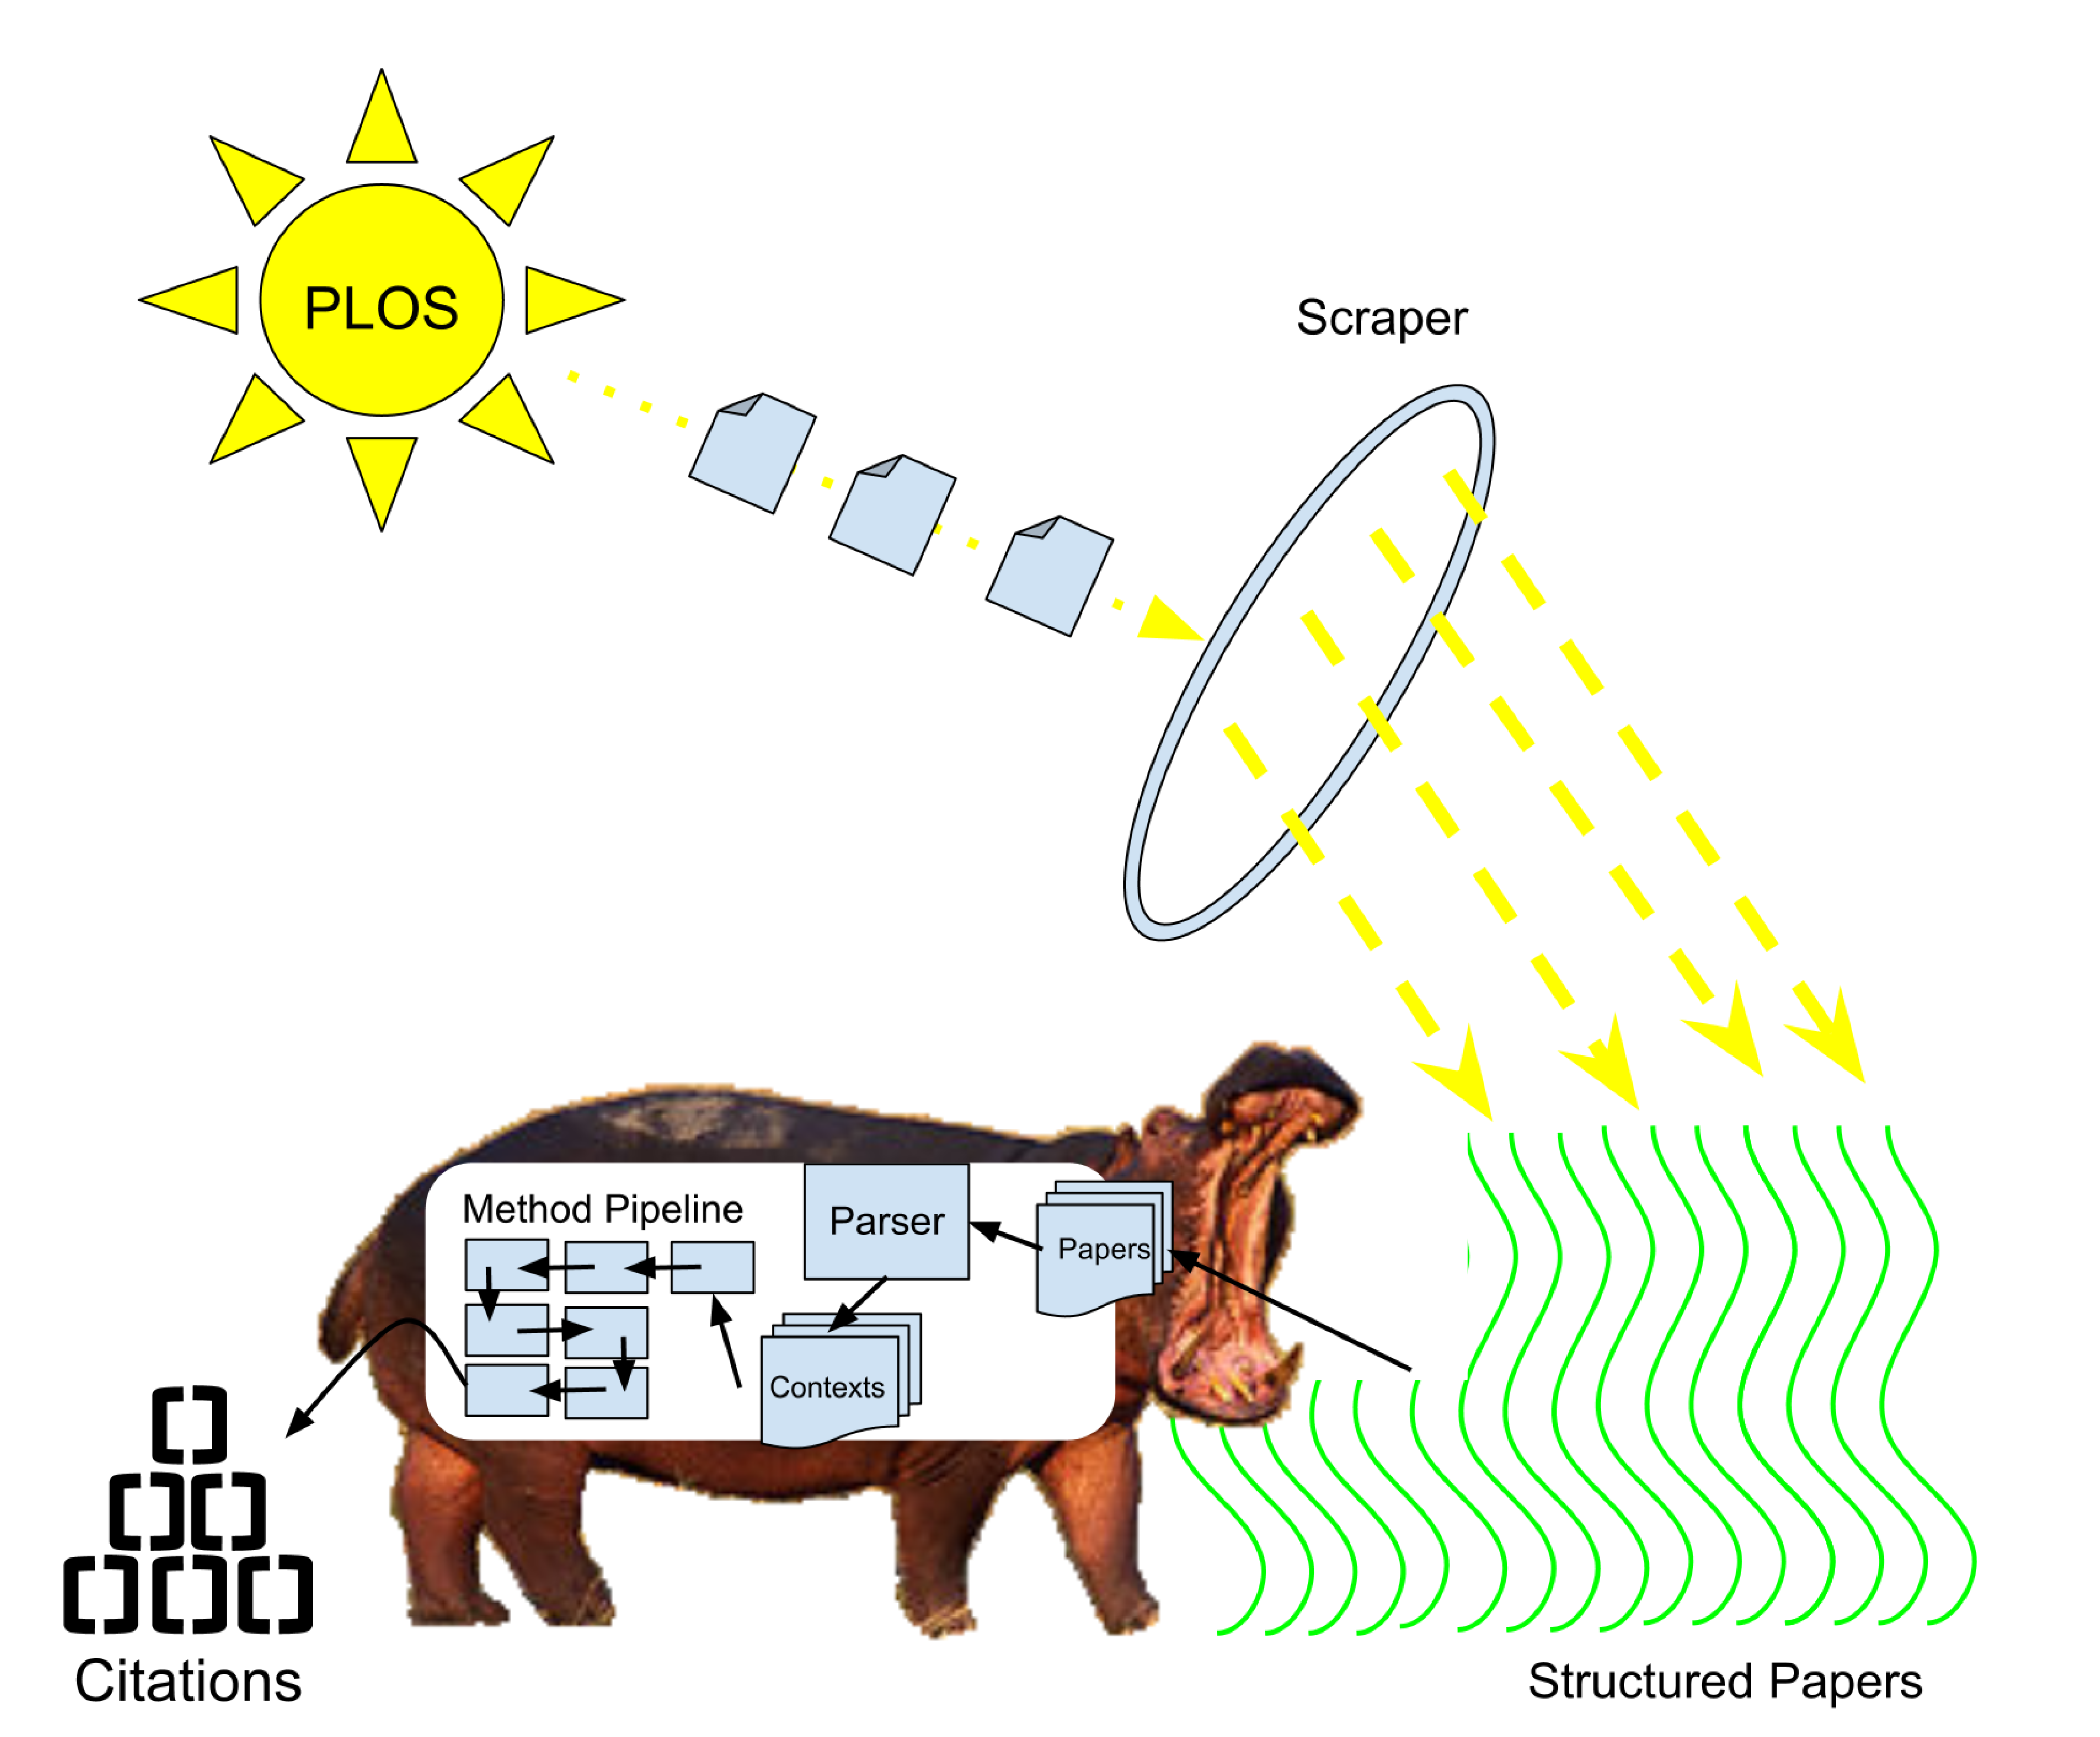
\includegraphics[width=\textwidth]{images/arch.eps}
        \caption{The Citeopotamus architecture overlaid on a hippopotamus.}
        \label{fig:arch}
\end{figure*}

\subsection{Scraper}\label{sec:scrape}
The scraper, written in python, extensively uses urllib2 and lxml.html. The
first task is to access a search landing page using urllib2. Each search result
page maintains 10 publications per page and links at the top
and bottom of the search page that lead to other search result pages. Each
publication located on a search result page is used as a root paper.
Each listing on the search result page contains metadata for the publication
listed such as title, author, and path to the HTML of the publication.
Since we are collecting this dataset programmatically, the HTML
version is easier to work with than a PDF version of the publication, which
would require OCR to extract text. Due to the structure of the page (which is
amazingly consistent), the HTML is parsed in the following sections:
\begin{itemize}
   \item Abstract
   \item Body sections and titles
   \item References
      \begin{itemize}
         \item Search pages for each references paper
         \item Pubmed page for each reference paper
         \item Abstract, Title, and Author for refererence paper from pubmed
      \end{itemize}
\end{itemize}

First, we extract the abstract text. This is made trivial with lxml's html
parser, specifically the cssselect and text\_content methods. Similarly, the
extraction of body section text and titles of publication is easily done.
Reference papers are more difficult to obtain due to the extra content that
must be fetched online. Each reference paper listing may or may not have a link
to a landing page listing various other sources where the publication may be
found. In cases where there is no link, then this listing is skipped and the
next one parsed. For cases where there is indeed a link, the pubmed source is
always picked and the provided pubmed URL to the publication is used to
retrieve the abstract, title, and authors for the reference paper. While pubmed
makes extraction of the abstract text somewhat difficult, it is solved through
the use of text\_content in python's lxml library, which grabs all text from
child nodes and removes HTML markup. As the necessary information for each
reference paper is retrieved, the reference paper is written out in the
appropriate directory location as mentioned below in section
\ref{sec:dir_structure}.

\subsubsection{Structure of Paper Text}\label{sec:text_structure}
If the paper text was generated from OCR, then the structure of the text was
left up to the OCR engine. However, papers scraped from PLOS were in HTML and
extra formatting can be inferred.

All text inside top-level $p$ tags can be inferred to be an entire paragraph
which was placed on a single line. The references section was separated from the
rest of the paper by a single line with only ``REFERENCES'' on it.
Additionally, the top of the text file listed ``TITLE:'', ``AUTHORS:'', and
extra information if accessible (which was not the case for PLoS Computational
Biology, specifically ``TERMS:'' and ``CATEGORIES:'').

\subsection{Structured Paper Directory Format}\label{sec:dir_structure}
The output of the scraper is a directory that contains information about the
root paper and all collected reference papers. To make all the
information easily accessible to anyone without imposing any arbitrary
restrictions, the structure of the data is enforced by directory structure.

The root directory is named using the root paper's title. Inside the root
directory is a ``references'' directory and four or five files, described
below. Inside the ``references'' directory are sub-directories for each
citation number in the root paper. The information for reference papers are
maintained in the appropriately numbered directory, such that a reference paper
``foo'', is the fourth citation (i.e. appears in the root paper as ``[4]'')
then information for paper ``foo'' is maintained in the directory ``4'' in the
root paper's ``references'' directory. A missing directory
means that the scraper could not collect that reference's information.

Every directory that represents a paper will have at most four files:
\begin{itemize}
   \item \textbf{meta.txt}\footnotemark[1]{} -- Contains the title, authors,
                                                tags, categories, and abstract.
                                                This is the only file required
                                                for every paper directory.
   \item \textbf{paper.txt}\footnotemark[1]{} -- The text version of the paper.
                                                 This file is required for the
                                                 root paper.
   \item \textbf{refs.txt}\footnotemark[1]{} -- Only the references that appear
                                                at the bottom of the paper.
                                                This information is duplicated
                                                in paper.txt, but placed here
                                                for convenience.
   \item \textbf{paper.pdf} -- The pdf version of the paper.
   \item \textbf{paper.html} -- The HTML version of the publication. This is
                                grabbed should the paper need to be re-parsed.
\end{itemize}

\footnotetext[1]{These files \textbf{are required} for our implementation to work}

A sample directory structure can be seen in Figure \ref{fig:tree}.

\begin{figure}[ht]
   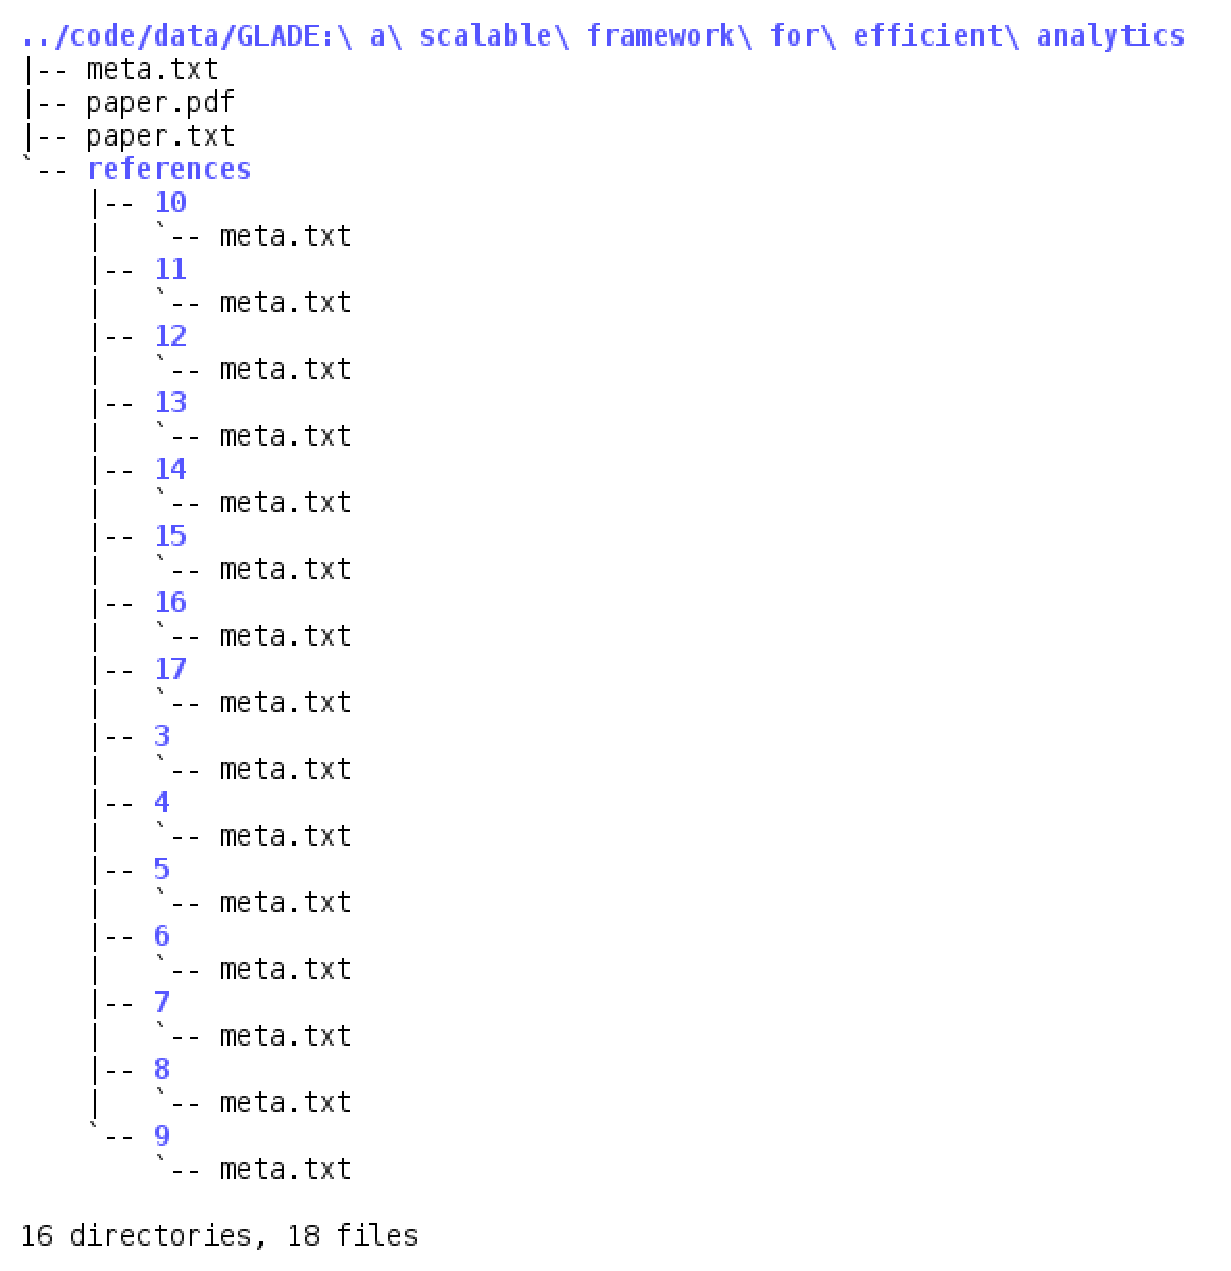
\includegraphics[width=\columnwidth]{images/tree.eps}
        \caption{The structure of a paper directory.}
        \label{fig:tree}
\end{figure}

\subsection{Citer}\label{sec:archCiter}
The citer begins by attempting to parse a directory structure into a structured collection of papers.
The citer then pre-processed each paper and generates a set of contexts (see Section \ref{sec:context}) for each citation in each
root paper.

After all of the contexts are generated, those contexts are fed into the Method Pipeline. In this pipeline are all the methods (see Section \ref{sec:methods})
that operate on the contexts to try and generate citations. Each citation in put through each method one at a time. If any method emits a value, then the pipeline
it short circuited and the emitted value is used as the citation. Because of this short circuiting behavior, the methods in the pipeline are ordered by approximate
precision. That is, all of the methods that rarely miss (regardless of how many citations they correctly place) are moved to the front of the pipeline.
As a citation travels through the pipeline, its citation becomes more and more uncertain.

\section{Parsing}\label{sec:parsing}
Because of its recursive nature, parsing the directory structure itself is rather simple.
Parsing the text of a paper however, can be quite complex.

\subsection{OCR}
Before any parsing can be done a paper, it must first be converted to a plain text (UTF-8) format.
Since PLOS provides most of their papers in an HTML format, this only had to be done off-line for a few
papers. After looking at many alternatives, we chose to use ABBYY Finereader 10\cite{abbyy}. This
is a commercial OCR product, and requires a licence to use.

ABBYY Finereader clearly outperformed all of the other OCR products we tried. It is especially
good at maintaining and recognizing formatting. Many other OCR products failed to correctly parse
two-column formats and thus generated unusable output.

\subsection{Transformations}\label{sec:transforms}
Before parsing the text of the paper, we had to make some global transformation on the paper.
Most of these transformations were done with simple regular expressions.

\subsubsection{Multiple Citations}
It is not unheard of for authors to make multiple citations within the same brackets: $$[1, 2]$$
These have to be parsed out and replaced with individual citations next to each other: $$[1][2]$$

\subsubsection{Ranges}
It is very common for authors to cite entire ranges at a time: $$[1] - [3]$$
This is especially seen when an author is referencing background material. These ranges must be expanded out to
the fill list of citations: $$[1][2][3]$$

\subsubsection{False Positive Sentence Enders}\label{sec:fpEnders}
Being able to split up paragraphs into sentences is very important to the Citeopotamus system.
We first tried to use NLTK's \textit{PunktSentenceTokenizer}. However, this did not seem to work well.
It seemed to have a problem with some of the symbols used in academic papers, such as the square brackets around
citations. To combat the punctuation tokenizing problem, we decided to only split sentence on periods, question marks, and
exclamations points. Additionally, we replaced common false positive sentence enters i.e.
$$i.e. => \_ie\_$$
$$dr. => \_dr\_$$
$$0.05 => \_0\_05\_$$

Using this tactic, there is a chance that a real sentence ender is replaced. However, this will still
include the original sentence in the result and the original sentence will still be located closer to the
citation that the incorrectly included sentence. Missing a significant portion of a sentence would be a much more
grievous error because then the context required to identify the citation may be missing.

\subsection{Contexts}\label{sec:context}
Contexts are the core of the Citeopotamus system. A ``context'' is just the words surrounding the citation.
Deciding which words to include in a context is very important. We use three different types of contexts that are meant for different
levels of precision. The contexts that include more words tends to be less precise and will therefore appear later in the pipeline.
However, these larger contexts have access to more information than the smaller ones and can sometimes makes guesses that are impossible
(outside of random) to the smaller contexts.

\subsubsection{Paragraph}
The largest of the contexts. We do not consider anything larger because it is very rare for an author to include information about a citation
outside of the paragraph that the citation is in (not including parsing or OCR formatting errors). Paragraphs are easy to parse because the
scraper puts one paragraph per line.

\subsubsection{Sentence}
Sentence level contexts contain just the sentence that the citation was main in. As discussed in Section \ref{sec:fpEnders},
sentence context is parsed just by splitting the paragraph on sentence ending punctuation after false positives have been replaced.

\subsubsection{Clause}
Clause context is the smallest and most complex context. The purpose of this context is to capture the clause that the citation was made in.
There are two parts to parsing this context: looking for parenthesis and walking backwards in the sentence.

We will use the following actual sentence as a running example:
\begin{quote}
In previous work, the Guyton models were modularized and reimplemented in Fortran, C++ (M2SL \textbf{[]}), and Simulink \textbf{[]}.
\end{quote}

When trying to find the context of the first citation, we recognize that it is surrounded by parenthesis.
We take the parenthesis as a hint the that content inside the parenthesis is more related to the citation than the surrounding words.

If there are no parenthesis surrounding the citation (as with the second citation), then we begin walking backwards in the sentence from the citation.
We will continue walking backwards in the sentence until we find:
\begin{enumerate}
   \item The beginning of the sentence.
   \item Another citation.
   \item A character that may break a clause: '[', ']', '.', ',', ';', ':', '!', '"', '?', or '-'.
\end{enumerate}

We do not include the words that appear after the citation because we want to avoid a clause context expanding into a sentence context and
in English, information about a reference is usually presented before the citation.

Our example would generate two clause contexts:
\begin{quote}
M2SL
\end{quote}

\begin{quote}
and Simulink
\end{quote}

Note that both cases generate contexts that contain the name of the product featured in the paper and no erroneous information. Whereas the
sentence context not only contains both produces, but a slew of other seemingly important words: ``Guyton'', ``Fortran'', and ``C++''.

\section{Methods}\label{sec:methods}
All of our current methods use the same algorithm for determining the most appropriate reference for a citation.
The difference in methods is the context and reference material that they choose to use.
We use the full cross-product of contexts and reference materials in the final system.

\subsection{Reference Material}
The reference material is the text that is associated with the reference.
The reference material that has the highest similarity to the context and surpassing the threshold is
used as the guess for that citation.
We use two different kinds of reference material: \textit{Reference Only} and \textit{Abstract}.

\subsubsection{Reference Only}
This reference material contains only information that is found in the reference section at the bottom of a paper.
Note that for ease of parsing we take this information from the reference's meta information, and not the actual paper. However given
some knowledge about how the references are formatted, it is trivial to parse out the title and authors.

For this reference material we take the all the author names longer than two characters and the paper title.
These words are then treated as unigrams.

\subsubsection{Abstract}
This reference material starts with the reference paper's abstract. However taking the entire abstract would include too many
useless features, so we try to narrow it down some. We begin by removing all the stopwords from the abstract. We use
the stopword list from the Onix Text Retrieval Toolkit\cite{stopwords}.

The first set of features that we grab are all of the capital words in the abstract. The main idea here is to grab
most of the ``important words'' in an abstract. A pronoun would be a very important word. The drawback of this method is that
is will usually grab the first word in a sentence. This is mitigated by removing stopwords. The first word in a sentence
is often the subject or a stopword (``The'', ``A'', etc).

The second set of features we collect are the bigrams of the abstract, after stopword removal.

To supplement the unigrams, we include any word that appears in any position of $\geq25\%$ of the bigrams.

\subsubsection{Unique Sets}
To help distinguish between the different references, we take all of the parsed reference material features and
keep only features that appear in no more than two of the references. This way we can keep features that are somewhat
unique, but get rid of features that occur too much.

\subsection{History}
It is rare for an author to cite the same paper twice in a paragraph. Even more rare for
an author to cite the same paper twice in a sentence, and almost unheard of for an author to cite the
same paper twice in the same clause. However, it is very common for there to be multiple citations
made in the same context. To combat this, every method remembers every citation that it has given
for each context in each paper. Since a method can remember its history, it can avoid making the
same guess for a context.

\subsection{Context Similarity}
To compare the similarity between a context and the reference material, we use a Jaccardian Distance\cite{jaccard}.

\section{Evaluation}\label{sec:eval}
To evaluate our system, we find the total number of references that we have successfully placed.

Given $n$ papers $(p_{1}, p_{2}, p_{3} ..., p_{n})$. We will let $RF(p_{i})$ be the number of references
for which we have full contextual information on and let $RT(p_{i})$ is the number of references
that were correctly placed in the paper $p_{i}$.

Then we let our accuracy be:
$$Accuracy = \frac{\sum_{i = 1}^{n} RF(p_{i})}{\sum_{i = 1}^{n} RT(p_{i})}$$

\subsection{Adjacent Citations}
While evaluating the results of a run, it is important to take into account \textit{adjacent citations}.
These are citations that appear right next to each other without any content separating each other (``[][]'' and ``[], []''
are both adjacent citation). We run into this situation often because we purposefully generate adjacent citations (see
Section \ref{sec:transforms}).

To deal with adjacent citations, we allow a citation guess to appear in any one of the adjacent positions.

\section{Results}\label{sec:results}
Because there are no other programs that attempt to do automated citation placement, we have no baseline to compare against.
A random baseline would be inappropriate for this situation since there are is such a small chance of getting a correct
citation when a paper has 50+ references.

\begin{table}[H]
\centering
\begin{tabular} { l | c | r }
\hline\hline
        {\bf $\sum_{i = 1}^{n} RF(p_{i})$} & {\bf $\sum_{i = 1}^{n} RT(p_{i})$} & {\bf Accuracy} \\[0.5ex]
\hline
        ? & ? & ? \\[0.5ex]
\end{tabular}
\caption{Results}
\label{tab:results}
\end{table}

\section{Future Work}\label{sec:future}
There are many opportunities for future work in this project.
Improving the actual implementation and increasing the scope of this project are both very plausible.

\subsection{Implementation Improvements}

\subsubsection{Parsing and Scraping}
Parsing is essential to the Citeopotamus system. If a context is improperly parsed, then everything else around that citation falls apart.
A spot check of papers that perform poorly (under 10\% accuracy) reveals that many of these these papers have many incorrectly parsed contexts.
Some of these errors come from an error in parsing like missing a false positive sentence ender. However, most of these errors appear to
come from difficulties scraping the paper. We believe that irregularities in the paper's HTML causes poor formatting of the resulting
plain text paper and therefore causes parsing errors.

\subsubsection{Pipeline Uncertainty}
As mentioned in Section \ref{sec:archCiter}, the further a citation moves into the pipeline the more uncertain its guessed citation becomes.
Incorporating this uncertainty into the information provided to the user can be very useful in a real-world system.

\subsubsection{Context Similarity}
Our current method for determining context similarity is very simplistic. A more complex algorithm that takes into account a word's distance to the
citation may perform better.

\subsubsection{Important Words}
Currently, we very simplistically find words that we believe to be important in a sentence. Because these are the words that
we compare to the reference material, choosing these words is key to guessing a citation. A very simple way to try and improve on this
would be to use a parts of speech tagger to find all the proper nouns in a context. We did not use POS tagging because
the NLTK POS taggers take too much time to run for the amount of gain it provides.

Using synonym can also help finding important words.

\subsection{Scope Increase}
The first step to increasing the scope of this project would be to tackle the other problem discussed in the Introduction,
guessing a citation given no information about where the citation appears.

Once that step is complete, a citation placement engine can be turned into a citation recommendation system.
The end goal would be a system where you can input your entire paper, and the system would recommend what papers
you should be citing. This can be an invaluable tool when writing related works and background sections.

\section{Related Work}\label{sec:related}
We were unable to find any related work on recommending citations given a spot for a citation to go. Unlike the problem of recommending citations for a paper. Copious amounts of work already exists on the topic. With several different approaches. One of the most common was using models to compare a paper and the rest of the dataset. Some of the models used includes translation models, probabilistic models, and several forms of LDAs.\cite{cite1, cite2, cite3} The next most common group of solutions was to use citations graphs to recommend missing citations.\cite{cite6} One group extended the notion of graphs and included metadata to help filter out results.\cite{cite4} One of the most 
interesting and unique approaches was to not look at co-citations but to look at co-accesses via logs like HTTP access records.\cite{cite7}
Another interesting approach used collaborative filtering to let communities help decide citations.\cite{cite8} For more related work in
citation recommendation we recommend the survey by McNee et al. they go into a lot of depth on the problem and common pitfalls.\cite{cite5}

\section{Conclusion}\label{sec:conclusion}
We have found that automatic citation placement is a difficult, but doable problem.

\section{Thanks}
We thanks the folks at PLOS for providing the source of our dataset. Without them this would of been a lot harder.

\bibliographystyle{acm}
\bibliography{refs}

\end{document}
